% THE DEGRADATION LADDER. Channel count against what survives, drawn as a
% ladder rather than a table because the point is that the system steps down
% rather than stopping.
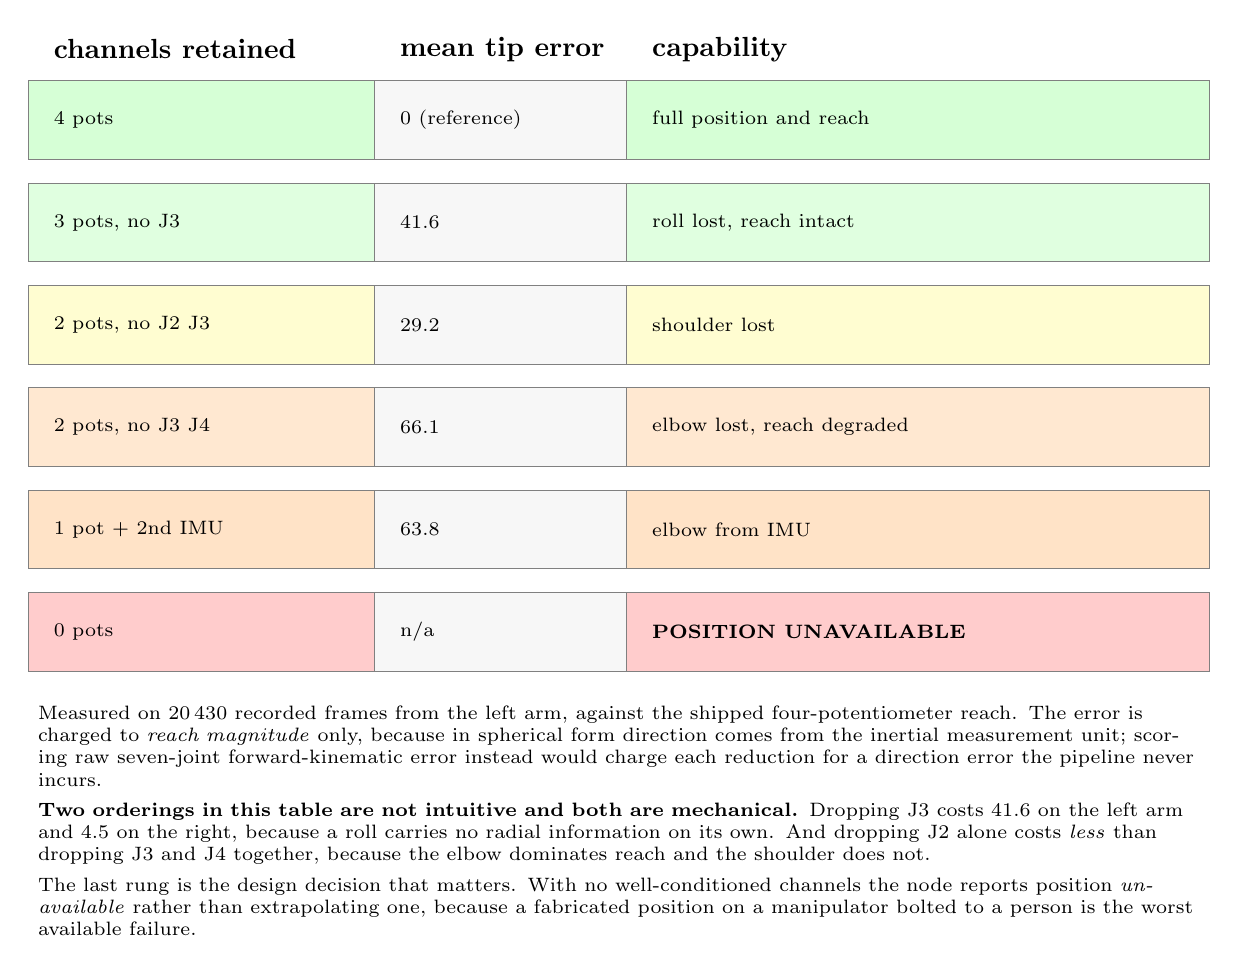
\begin{tikzpicture}[x=1mm, y=1mm, font=\scriptsize]

\foreach \i/\pots/\err/\lab/\col in {
  0/{4 pots}/{0 (reference)}/{full position and reach}/{green!16},
  1/{3 pots, no J3}/{\SI{41.6}{\milli\metre}}/{roll lost, reach intact}/{green!12},
  2/{2 pots, no J2 J3}/{\SI{29.2}{\milli\metre}}/{shoulder lost}/{yellow!18},
  3/{2 pots, no J3 J4}/{\SI{66.1}{\milli\metre}}/{elbow lost, reach degraded}/{orange!18},
  4/{1 pot $+$ 2nd IMU}/{\SI{63.8}{\milli\metre}}/{elbow from IMU}/{orange!22},
  5/{0 pots}/{n/a}/{\textbf{POSITION UNAVAILABLE}}/{red!20}}
{
  \pgfmathsetmacro{\y}{-\i*13}
  \draw[fill=\col, draw=black!50] (0,\y) rectangle (44,\y+10);
  \node[anchor=west] at (2, \y+5) {\pots};
  \draw[fill=gray!6, draw=black!50] (44,\y) rectangle (76,\y+10);
  \node[anchor=west] at (46, \y+5) {\err};
  \draw[fill=\col, draw=black!50] (76,\y) rectangle (150,\y+10);
  \node[anchor=west] at (78, \y+5) {\lab};
}
\node[anchor=west, font=\bfseries] at (2, 14) {channels retained};
\node[anchor=west, font=\bfseries] at (46, 14) {mean tip error};
\node[anchor=west, font=\bfseries] at (78, 14) {capability};

\node[anchor=west, text width=148mm, align=left] at (0, -84)
  {Measured on 20\,430 recorded frames from the left arm, against the shipped
   four-potentiometer reach. The error is charged to \emph{reach magnitude}
   only, because in spherical form direction comes from the inertial
   measurement unit; scoring raw seven-joint forward-kinematic error instead
   would charge each reduction for a direction error the pipeline never
   incurs.\\[3pt]
   \textbf{Two orderings in this table are not intuitive and both are
   mechanical.} Dropping J3 costs \SI{41.6}{\milli\metre} on the left arm and
   \SI{4.5}{\milli\metre} on the right, because a roll carries no radial
   information on its own. And dropping J2 alone costs \emph{less} than
   dropping J3 and J4 together, because the elbow dominates reach and the
   shoulder does not.\\[3pt]
   The last rung is the design decision that matters. With no
   well-conditioned channels the node reports position \emph{unavailable}
   rather than extrapolating one, because a fabricated position on a
   manipulator bolted to a person is the worst available failure.};
\end{tikzpicture}
